\documentclass{article}
\usepackage[a4paper, margin=0.75in]{geometry}
\usepackage{titlesec}
\usepackage{fontspec}
\usepackage{multicol}
\usepackage{tikz}
\usetikzlibrary{arrows.meta, positioning}


\titleformat{\subsubsection}[block]{\normalfont\normalsize\bfseries}{\thesubsubsection}{1em}{}

\setcounter{secnumdepth}{3}
\setcounter{tocdepth}{3}

\usepackage{preamble04}

\titleformat{\section}
{\normalfont\Large} 
  {\thesection}{1em}{}

\begin{document}



\subsection*{Journal Entry: Cash Sales}

\vspace{1em}

\begin{center} 
\begin{tabular}{@{} l l l l r @{}}
\toprule
& \textbf{Account Title} & \textbf{Category} & \textbf{Explanation} & \textbf{Amount (\$)} \\
\midrule
Dr & Cash & Asset & Cash increased & \hfill 1,000 \\
 & \quad  & \\
Cr & Sales Revenue & Income & Sales increased& \hfill (1,000) \\
\bottomrule
\end{tabular}
\end{center}
\vspace{1em}
\textit{Journal Entry: Cash Sales}

\vspace{1em}

\begin{center} 
\begin{tabular}{@{} l l l l r @{}}
\toprule
& \textbf{Account Title} & \textbf{Category} & \textbf{Explanation} & \textbf{Amount (\$)} \\
\midrule
Dr & Trade Receivables & Asset & Trade Receivables increased & 1,000 \\
 & \quad  & \\
Cr & Sales Revenue & Income & Sales increased& (1,000) \\
\bottomrule
\end{tabular}
\end{center}
\vspace{1em}
\textit{Journal Entry: Trade Receivables}

\begin{center} 
\begin{tabular}{@{} l l l l r @{}}
\toprule
& \textbf{Account Title} & \textbf{Category} & \textbf{Explanation} & \textbf{Amount (\$)} \\
\midrule
Dr & Sales as Sales returns & Income & Sales decreased & 1,000 \\
 & \quad  & \\
Cr & Trade Receivables & Asset & Receivables decreased & (1,000) \\
\bottomrule
\end{tabular}
\end{center}
\vspace{1em}
\textit{Journal Entry: Sales Return}

\begin{center} 
\begin{tabular}{@{} l l l l r @{}}
\toprule
& \textbf{Account Title} & \textbf{Category} & \textbf{Explanation} & \textbf{Amount (\$)} \\
\midrule
Dr & Bank/Cash & Asset & Bank/Cash increased & 1,000 \\
 & \quad  & \\
Cr & Trade Receivables & Asset & Receivables decreased & (1,000) \\
\bottomrule
\end{tabular}
\end{center}
\vspace{1em}
\textit{Journal Entry: Receipts from customers}


\begin{center} 
\begin{tabular}{@{} l l l l r @{}}
\toprule
& \textbf{Account Title} & \textbf{Category} & \textbf{Explanation} & \textbf{Amount (\$)} \\
\midrule
Dr & Purchases & Expense & Purchases increased & 1,000 \\
 & \quad  & \\
Cr & Cash/Bank & Asset & Cash decreased & (1,000) \\
\bottomrule
\end{tabular}
\end{center}
\vspace{1em}
\textit{Journal Entry: Cash purchases}


\begin{center} 
\begin{tabular}{@{} l l l l r @{}}
\toprule
& \textbf{Account Title} & \textbf{Category} & \textbf{Explanation} & \textbf{Amount (\$)} \\
\midrule
Dr & Purchases & Expense & Purchases increased & 1,000 \\
 & \quad  & \\
Cr & Trade Payables & Liability & Payables increased & (1,000) \\
\bottomrule
\end{tabular}
\end{center}
\vspace{1em}
\textit{Journal Entry: Credit purchases}


\begin{center} 
\begin{tabular}{@{} l l l l r @{}}
\toprule
& \textbf{Account Title} & \textbf{Category} & \textbf{Explanation} & \textbf{Amount (\$)} \\
\midrule
Dr & Trade Payables & Liability & Payables decreased & 1,000 \\
 & \quad  & \\
Cr & Purchases & Expense & Purchase decreased & (1,000) \\
\bottomrule
\end{tabular}
\end{center}
\vspace{1em}
\textit{Journal Entry: Purchase Returns}

\begin{center} 
\begin{tabular}{@{} l l l l r @{}}
\toprule
& \textbf{Account Title} & \textbf{Category} & \textbf{Explanation} & \textbf{Amount (\$)} \\
\midrule
Dr & Trade Payables & Liability & Payables decreased & 1,000 \\
 & \quad  & \\
Cr & Bank/Cash & Asset & Cash decreased & (1,000) \\
\bottomrule
\end{tabular}
\end{center}
\vspace{1em}
\textit{Journal Entry: Payment to Suppliers}


\subsection{Irrecoverable Debts}

\begin{center} 
\begin{tabular}{@{} l l l l r @{}}
\toprule
& \textbf{Account Title} & \textbf{Category} & \textbf{Explanation} & \textbf{Amount (\$)} \\
\midrule
Dr & Irrecoverable debt expenses account & expenses & Irrecoverable debt expenses increased & 1,000 \\
 & \quad  & \\
Cr & Trade Receivables & Asset & Receivables decreased & (1,000) \\
\bottomrule
\end{tabular}
\end{center}
\vspace{1em}
\textit{Journal Entry: Payment to Suppliers}

\subsubsection{Subsequent Recovery of Irrecoverable Debt}

Step 1: Reverse the irrecoverable debt write-off 

\begin{center} 
\begin{tabular}{@{} l l l l r @{}}
\toprule
& \textbf{Account Title} & \textbf{Category} & \textbf{Explanation} & \textbf{Amount (\$)} \\
\midrule
Dr & Receivables & Asset & Receivables increased & 1,000 \\
 & \quad  & \\
Cr & Irrecoverable debts expense account & Expense & Irrecoverable debts expensed decreased & (1,000) \\
\bottomrule
\end{tabular}
\end{center}
\vspace{1em}
\textit{Journal Entry: Payment to Suppliers}

Since the balance owed has been paid, the amount is not irrecoverable. Therefore, an adjustment to reverse te earlier write-off is made. 

Step 2: Record the Receipts

\begin{center} 
\begin{tabular}{@{} l l l l r @{}}
\toprule
& \textbf{Account Title} & \textbf{Category} & \textbf{Explanation} & \textbf{Amount (\$)} \\
\midrule
Dr & Bank & Asset & Bank increased & 1,000 \\
 & \quad  & \\
Cr & Receivables & Asset & Receivables decreased & (1,000) \\
\bottomrule
\end{tabular}
\end{center}
\vspace{1em}
\textit{Journal Entry: Payment to Suppliers}

Therefore, the net effect of the above two entries is Dr\. Bank, Cr. Irrecoverable debits expense account. 


\subsection{Allowance for irrecoverable debts}

\begin{enumerate}[label=\arabic*, resume] 
    \item Calculate the closing allowance for the allowance for irrecoverable debts at the year-end. 
    \item Calculate the difference between the closing allowance and the opening allowance (brought forward from the previous accounting period) 
    \item The difference is posted as a journal entry to the allowance for irrecoverable debits ledger. The corresponding account is the irrecoverable debts expense account. 
\end{enumerate}

If the closing allowance is more than the opening allowance, the double entry to record the adjustment is: 

\begin{center} 
\begin{tabular}{@{} l l l l r @{}}
\toprule
& \textbf{Account Title} & \textbf{Category} & \textbf{Explanation} & \textbf{Amount (\$)} \\
\midrule
Dr & Irrecoverable debts expense & Expense & Bank debt increased & 1,000 \\
 & \quad  & \\
Cr & Allowance for irrecoverable debts & Asset & Receivables decreased & (1,000) \\
\bottomrule
\end{tabular}
\end{center}
\vspace{1em}
\textit{Journal Entry: Payment to Suppliers}

Since it has been identified that the closing allowance is more than the opening allowance, the difference is posted as an irrecoverable debts expense in the statement of profit or loss (in the same way as an irrecoverable debt written off). 

If the closing allowance calculated is less than the opening allowance, the double entry to record the adjustment is: 


\begin{center} 
\begin{tabular}{@{} l l l l r @{}}
\toprule
& \textbf{Account Title} & \textbf{Category} & \textbf{Explanation} & \textbf{Amount (\$)} \\
\midrule
Dr & Allowance for irrecoverable debts & Asset & Receivables increased & 1,000 \\
 & \quad  & \\
Cr & Irrecoverable debt expense & Expense & Irrecoverable debts expense decreased & (1,000) \\
\bottomrule
\end{tabular}
\end{center}
\vspace{1em}
\textit{Journal Entry: Payment to Suppliers}

Since the closing allowance is less than the opening allowance, the difference is posted to decrease the irrecoverable debt expense. The reduced expense will be shown in the statement of profit or loss.

(Note – while the Allowance for irrecoverable debts is described as an asset account, it is a negative asset, as it reduces the value of trade receivables in the statement of financial position.)

\subsection{Inventory} 

The record of inventory and cost of goods sold are made at the end of the year using journals. The objective of the double entries is to:

    Ensure the Inventory account reflects the closing inventory valuation
    Cost of goods sold account is created and reflects the correct amount

To achieve these objectives, there are three double-entry steps to make:

1. Remove the Opening Inventory

Opening inventories are removed and transferred to the Cost of goods sold account. This entry is necessary because the opening inventories are now used to generate sales in the current accounting period.

\begin{center} 
\begin{tabular}{@{} l l l l r @{}}
\toprule
& \textbf{Account Title} & \textbf{Category} & \textbf{Explanation} & \textbf{Amount (\$)} \\
\midrule
Dr & Cost of goods sold & Expense & Opening inventory cost now included as expenses & 1,000 \\
 & \quad  & \\
Cr & Inventory & Asset & Inventory decreased & (1,000) \\
\bottomrule
\end{tabular}
\end{center}
\vspace{1em}
\textit{Journal Entry: Payment to Suppliers}

The cost of opening inventories is reflected as a current-year expense in the Statement of Profit or Loss.

2. Close off the Purchases Account

A business makes purchases for inventory for resale. The cost is debited to the Purchases account and credited to cash/payables at the point of purchase. At year-end, the amount in the Purchases account is closed off and transferred to the Cost of Goods Sold.


\begin{center} 
\begin{tabular}{@{} l l l l r @{}}
\toprule
& \textbf{Account Title} & \textbf{Category} & \textbf{Explanation} & \textbf{Amount (\$)} \\
\midrule
Dr & Cost of goods sold & Expense & Purchases is transferred to COGS & 1,000 \\
 & \quad  & \\
Cr & Purchases & Expense & Purchases is closed off & (1,000) \\
\bottomrule
\end{tabular}
\end{center}
\vspace{1em}
\textit{Journal Entry: Payment to Suppliers}


3. Post the Closing Inventory

The balance in the inventory account at year-end should reflect the value of closing inventory. The closing balance is presented in the statement of financial position as a current asset.

Since closing inventories are items purchased that are not sold in the accounting period, their cost should not be reflected as an expense in the Cost of goods sold account (SPL). Therefore, the value of closing inventory is transferred out of expenses and reflected as Closing inventory in the Statement of Financial Position.

\begin{center} 
\begin{tabular}{@{} l l l l r @{}}
\toprule
& \textbf{Account Title} & \textbf{Category} & \textbf{Explanation} & \textbf{Amount (\$)} \\
\midrule
Dr & Inventory & Asset & Inventory is increased & 1,000 \\
 & \quad  & \\
Cr & Cost of goods sold & Expense & Costs decreased & (1,000) \\
\bottomrule
\end{tabular}
\end{center}
\vspace{1em}
\textit{Journal Entry: Payment to Suppliers}

The value of closing inventory will be next year's opening inventory value.





% Chapter 1 
% \section{Introduction to the Regulatory Framework}


The primary roles of the International Accounting Standards Board and the International Sustainability Standards Board within the IFRS Foundation's governance structure are to develop and publish accounting standards and develop a baseline of sustainability-related disclouse standards.

Pubilc accountability refers to being subject to punishment or consequences in the case of failure or inadequate performance in carrying out tasks. In the case of IFRS standard-setting, they are held accountable by a monitoring board of public authorities (IFRS Foundation Monitoring Board). 


It is said that the "regulatory bodies do not have the power to force companies to comply" because, legally, they do not. IFRS is much more of a recommendation and implies that global adoption of their guidance can be ignored if chosen to do so.  


National accounting bodies can adopt IFRSs as standard or use it as a basis for developing guidance for their own country. They can also develop their own requirements but compare them to IFRSs to determine if their standards are sufficient. 


%%%%%%%%%%%%%%%%%%%%%%%%%%%%%%%%%%%%%%%%%%%%%%%%%%%%
%A. The Context and Purpose of Financial Statements
%%%%%%%%%%%%%%%%%%%%%%%%%%%%%%%%%%%%%%%%%%%%%%%%%%%%
% \input{note01.tex}

%%%%%%%%%%%%%%%%%%%%%%%%%%%%%%%%%%%%%%%%%%%%%%%%%%%%%%%%%%%%%
%B. The Qualitative Characteristics of Financial Information 
%%%%%%%%%%%%%%%%%%%%%%%%%%%%%%%%%%%%%%%%%%%%%%%%%%%%%%%%%%%%%
% \section{Elements of Financial Statements} 

Activity 1 

For each statement below, tate whether they are True or False. 

\begin{itemize}
    \item A Telephone that is used daily is a current asset.
    \item A machine used to create products is a tangible non-current asset. 
    \item A software licence that lalows a business to use specific software for a period of three years is a tangible non-current asset. 
    \item A truck a business uses to deliver goods to its customers is a tangible non-current asset. 
    \item Goods purchased by a business for resale to its customers are tangible non-current assets. 
\end{itemize}       

Activity 2 

In the following activity, classify the list of items into the elements of financial statements. 

\begin{itemize} 
    \item Shareholder's investment
    \item Computers 
    \item Bookkeeper's annual salary
    \item Warehouse 
    \item Unsold goods
    \item Overdraft with the bank
    \item Cash held at the bank
    \item Sales of goods for cash in the factor shop
\end{itemize} 

Activity 3 

The following activity presents different items that need to be classified under the correct heading in the financial statements. 

\begin{itemize} 
    \item Cost of selling furniture and other costs of running Coltom Co. 
    \item Buildings owned by Coltom Co. 
    \item The amount paid to purchase shares in Coltom Co. 
    \item Amounts Coltom Co. owes for goods and services purchased
    \item The income that Coltom Co. earns from selling furniture to its customers. 
\end{itemize} 


Match each example to the correct financial statement heading below: 

\begin{itemize}
    \item Assets in the Statement of Financial Position 
    \item Liabilities in the Statement of Financial Position 
    \item Equity in the Statement of Financial Position 
    \item Income in the Statement of Profit or Loss 
    \item Expense in the Statement of Profit or Loss
\end{itemize} 


Activity 4 

Classify the following items of expenditure as asset expenditures or expenses: 

\begin{enumerate} 
    \item \$27,000 on a new car. 
    \item \$1,800 road tax incorporated in the car's purchase price in (1) above.
    \item \$10,000 on a second-hand delivery van. 
    \item \$12,000 on refurbishing van in (3) above. 
    \item \$1,000 monthly rental of a vehicle. 
\end{enumerate} 

Activity 5

Rubin owns a business that sells office and computer equipment to corporate customers. His business operates from a warehouse and has a small fleet of delivery 
vehicles. Determine whether teh expenditures made by Rubin's business should be classified as expenses or asset expenditures. 

\begin{enumerate}
    \item Rubin's business has bought some laptops and speakers from its suppliers, which will be sold to its customer. 
    \item Rubin's accountant prepares its financial statements. She orderd a photocopier to make copies of her paperwork.
    \item Rubin's business is expanding, and he has rented a new wareouse. 
    \item Rubin ensures that all the vehicles have valid insurance. Each time he orders a new vehicle, he insures it immediately. 
    \item Goods are delivered to customers using one of the business's delivery vehicles. On the way back to the varehouse, the driver crashhes the side of the vehicle into the fence. The vehicle will need to be fixed to be used again. 
    \item Rubin's business orders a few new vehicles to keep up with customer orders. 
\end{enumerate}

\newpage

Activity 7

Match the equation to the corresponding rearranged accounting equation. 

\begin{table}[h!]
\centering
\begin{tabular}{|l|p{8cm}|l|}
\hline
\textbf{Transaction} & & \textbf{Duality Statement} \\
\hline
Assets & Opening capital + Profit for the period − Drawings & \\
\hline
Closing Net Assets & Closing net assets − Opening net assets + Drawings & \\
\hline
Opening Net Assets & Capital + Liabilities & \\
\hline
Closing Capital & Assets − Capital & \\
\hline
Liabilities & Closing net assets − Profit for the period + Drawings & \\
\hline
Profit for the period & Closing capital & \\
\hline
\end{tabular}
\caption{Transactions and Their Duality Statements}
\end{table}


Activity 8

What is the double entry to record the following transactions? 

\begin{enumerate}
    \item Starts the business by introducing cash.
    \item Purchases some equipment for cash. 
    \item Pays a supplier for some equipment bought on credt. 
    \item Purchases goods for resale on credit. 
    \item Purchases goods for resale for cash. 
    \item Sells goods on credit. 
    \item Sells goods for cash.
\end{enumerate}

%\section{The Regulatory and Conceptual Framework}


% What is the regulatory framework? 

Financial Accounting (Preparing financial statements) is governed by a set of standards called the International 
Financial Reporting Standards. These standards are mean't to ensure that financial statements accurately represent the 
financial conditions of a business, thus preventing their ability to mislead the stakeholders and shareholders interested in the 
business. 

% Who are they prepared by? 

The international accounting standards board issues these standards and give guidance upon them. The governance structure of setting standards is split into three areas, 
public accountability, independent standards setting and related activities and Governance strategy and oversight. The IFRS Foundation Board is responsible for public accountability, the IFRS trustee foundation 
is responsible for the Governance, strategy and oversight and the independent standard-setting is made up of the International Accounting Standards Board and the International Sustainability Standards Board. The Advisory Council is responsible for giving adivce to the trustees foundation, IASB 
and the ISSB. 


%\section{Accounting Systems and Maintaining Accounting Records}


The overall process for preparing financial statements include 6 steps.

\begin{enumerate} 
    \item Recording Business Transactions and 
    \item Verify the business transactions through financial documents based on the business transactions.
    \item Clasifying the Financial Documents into thir relevent general ledger accounts.
    \item Using the balances from the general ledgers to create the trial balance.
    \item Using the trial balance to create the financial statements. 
\end{enumerate}

\subsection{Business Transacitons} 

There are 6 main business transactions, (1) sales, (2) sale returns, (3) purchases, (4) purchase returns, (5) payments, (6) receipts.

\subsection{Financial Documents} 

There are 12 main financial documents, (1) Quotation, (2) Purchase Order, (3) Sales Order, (4) Delivery Note (Goods Despathed Note), (5) Goods Received Note (GRN) 
(6) Sales invoice (7) purchase invoice, (8) Credit Note, (9) Debit Note, (10) Statement of Account, (11) Remittance Advice, (12) Receipt. 


%%%%%%%%%%%%%%%%%%%%%%%%%%%%%%%%%%%%%%%%%%%%%%%%%%
%C. The Use of Double Entry and Accounting Systems
%%%%%%%%%%%%%%%%%%%%%%%%%%%%%%%%%%%%%%%%%%%%%%%%%%
%\section{5.1 Recording Business Transaction}

The recording business transactions module comprises of four subtopics. 

\begin{enumerate}
    \item Introduction to Recording Business Transactions 
    \item  Sales Tax
    \item Discount Received and Allowed
    \item  Bank Reconciliations
\end{enumerate}

\subsection{Introduction to Recording Business Transactions}

\subsubsection{Context: Types of Business Transactions}

Businesses engage in day-to-day operations to sustain the business' life cycle. The monetary value of these operations are referred to as business transactions. These transactions are important because they indiciate the company's financial health to the company and to parties interested in the business. 
In the FA exam, business transactions can be classified into i.) Cash and Credit Sales, ii.) Sale Returns, iii.) Cash and Credit Purchases, iv.) Purchase returns and v.) Petty Cash Transactions.

\subsubsection{Cash and Credit Sales}

A sale is the process of trading goods and services for money. A cash sale is a immediate transaction where goods and services are immediately exchanged for money while a credit sale refers to a future transaction where goods and services are exchanged for a future payment. Customers who purchased on credit should repay the business at the end of the current credit term. Customers who receive damaged or incorrect goods can return
them to the business. This is a sales return. When this occurs the business writes a credit note to reduce the value on the sales invoice. 

\subsubsection{Cash and Credit Purchases}

A purchase is the process of exchanging money for goods and services. A cash purchase is an immediate transaction where money is immediately exchanged for goods and services while a credit purchase is a future trasaction where goods and services are immediately received and money is exchanged at a later date. At the end of the credit term and credit purchase must be repaid in full. If the business receives damaged or incorrect goods they
can return them, with the supplier issuing a credit note to reduce the value on the preivously issued sales invoice. 

\subsection{Sales Tax} 

Sales tax is an indirect tax charged on goods and services sold or purchased, they are imposed by the government and tax authorities. Sales tax can be split into two classes, input tax and output tax. 

\begin{itemize}
    \item Input tax is sales tax charged on sales to customers 
    \item Output tax is the sales tax charged on purchases of goods and services.
\end{itemize}

If Output Tax $>$ Input tax, sales tax is considered a current liability and is owed to tax authorities.
If Input Tax $>$ Output tax, sales tax is considered a current asset, with the tax authorities owing the business. 


\subsection{Discounts Received and Allowed}

A discount is a reduction in the prices of goods, or services, below the price at which they would typically cost. Discounts can be classified into trade discounts 
or settlement discounts. Trade discounts are guaranteed discounts, and customers are expected to take advantage of these discounts. Therefore trade discounts offered are always 
considered when recognising transactions. Trade discounts on sales are called discounts received, while trade discounts on purchases are called discounts allowed.

\subsection{Bank Reconciliation}

A bank reconciliation is the process of indentifying and eliminating discrepencies between the bank statement's balance and the balance of the bank ledger account to ensure that both balances agree. 


A standing order is an instruction from the payer to the bank to pay a fixed amount on a predetermined date a third party. 

%\newpage

\begin{center}
\begin{tabular}{ |p{7cm}||p{7cm}|  }
    \hline
      \multicolumn{2}{|c|}{%
        \begin{tabular}{c}
            Big Dog Carworks Corp. \\
            \textbf{Balance Sheet} \\
            \textit{As of June 14\textsuperscript{th}, 20X6} 
        \end{tabular}
    } \\
    \hline 
    Resources (Assets) & Claims (Liabilities and Equity) \\ \\ 
        % Left: ASSETS table
    \begin{tabular}{p{3cm} r r}
        Cash & \$3,700 &  \\
        Accounts Receivable & \$2,000 \\
        % Add more assets as needed
        
        \textbf{Total Assets} &  & \textbf{\$3,700}
    \end{tabular}
    &
    % Right: CLAIMS table
    \begin{tabular}{p{3cm} r r}
        Capital & \$3,700 &  \\
        % Add more liabilities/equity as needed
        
        &  & \textbf{\$3,700}
    \end{tabular}
    \\
    \hline\end{tabular}
\end{center}



\begin{center}
\begin{tabular}{ |p{7cm}||p{7cm}|  }
    \hline
    \multicolumn{2}{|c|}{%
        \begin{tabular}{c}
            \textit{Big}

        \end{tabular}
    } \\
    \hline
    \\
    Resources (Assets) & Claims (Liabilities and Equity) \\ \\ 
    \begin{tabular}{p{3cm} r r}
        equipment & \$3,000.00  \\

        \textbf{Total Assets} & & \textbf{\$3,000.00}
    \end{tabular}
    &
    \begin{tabular}{p{3cm} r r}
        bank loan & \$6,000.00 \\

     & & \textbf{\$6,000.00}
    \end{tabular} \\
    \hline
\end{tabular}
\end{center}





\newpage
\begin{center}
\begin{tabular}{ |p{8cm}||p{8cm}|  }
    \hline
    \multicolumn{2}{|c|}{%
        \begin{tabular}{c}
Big Dog Carworks Corp. \\
Balance Sheet \\
At January 31 \\
\textit{2015}

        \end{tabular}
    } \\
    \hline
    \\
    Resources (Assets) & Claims (Liabilities and Equity) \\ \\ 
    \begin{tabular}{p{4cm} r r}
Cash & \$3,700.00 \\
Accounts receivable & \$2,000.00 \\
Prepaid insurance & \$2,400.00 \\
Equipment & \$3,000.00 \\
Truck & \$8,000.00 \\

        & & \textbf{\$19,100.00}
    \end{tabular}
    &
    \begin{tabular}{p{4cm} r r}
Bank Loan & \$6,000.00 \\
Accounts Payable & \$700.00 \\
Unearned revenue & \$400.00 \\
Share Capital & \$10,000.00 \\
Retained Earnings & \$2,000.00 \\

        & & \textbf{\$19,100.00}
    \end{tabular} \\
    \hline
\end{tabular}
\end{center}


%\input{note14.tex}

%%%%%%%%%%%%%%%%%%%%%%%%%%%%%%%%%%%%%
%D. Recording Transactions and Events
%%%%%%%%%%%%%%%%%%%%%%%%%%%%%%%%%%%%%
%\chapter{Recording Transactions and Events}

\section{IAS 37 Provisions, Contingent Liabilities and Contingent Assets}

\subsection{Provisions}

(IAS37) A provision is a liability of uncertain timing or amount and should be recognised when all the following criteria is satisified:

\subsubsection{Recognition Criteria}

Provisions are recognised upon the satisifaction of three criteria: 

\begin{enumerate}
    \item A present obligation exists due to a past event.
    \item An outflow of economic resources to settle the obligation is probable, meaning that there is a greater than 50\% chance of it occuring.
    \item A reliable estimate of the obligation can be made.
\end{enumerate}

If any of the above conditions are not fulfilled, a provision must not be recognised.
The main difference between a provision and a liability is the extent of uncertainty involved. IAS37 states that the amount of a provision should be equal to "the best estimate of the 
expenditure required to settle the present obligation at the end of the reporting period". 


The amount of the provision must be the best estimate of the expenditure required to settle the obligation concerned. This is of course a matter of judgement and may require advice from independent experts. Note that: 

\begin{enumerate}[a.]
    \item The "best estimate" of the required expenditure is the amount that the entity would rationally pay to settle the obligation or transfer it to a third party. 
    \item If the effect of the time value of money is material, the amount of a provision should be calculated as the present value of the expenditure required to settle the obligation. 
    \item Future events that may affect the amount required to settle an obligation should be taken into account when measuring a provision, so long as there is sufficient objective evidence that these events will occur. For instance, the estimated costs of cleaning up environmental damage might be reduced by anticipated changes in technology. 
\end{enumerate}

If a single obligation is being measured and there are several possible outcomes, the best estimate of the required expenditure is usually the cost of the most likely outcome.

But if most of the other possible outcomes would involve a higher cost, the best estimate of the expenditure will be a higher amount. Similarly, if most of the other possible outcomes would involve a lower cost, the best estimate of the
expenditure will be a lower amount.

In cases where a provision relates to a large population of items, the amount of the provision should be estimated by calculating the "expected value" of the obligation at the
end of the reporting period. This statistical method of estimation involves weighting all possible outcomes by their associated probabilities.

Example 1: 

In 20X6, Benedict was sued for damages by a significant customer for breach of contract. 
In March 20X7, the court ruled in favour of the customer but deferred its ruling on the number 
of damages until June. For legal advice in defence of this claim, Benedict paid \$15,000 in 20X6;
a further \$20,000 has been incurred to date (to be paid once the matter is settled in June), and Benedict expects 
to pay an additional \$10,000 before the case is wholly settled.

Benedict’s legal adviser thinks that Benedict will be required to reimburse the customer's legal costs, which he estimates will be as much as 
Benedict’s. Based on the level of damages claimed, he also believes these are likely to be in the region of \$250,000 to \$300,000.

Analysis of best estimate:

Benedict should provide for the following: 

\begin{itemize}
    \item its legal costs incurred after the end of the reporting period (\$15,000 incurred in 20X6 is already expensed, so not considered in calculating the provision.)
    \item the best estimate of the customer's legal costs 
    \item the best estimate of the damages. This is the most subjective. As the estimated range of the outcome is relativialy narrow, any amount in this rangce may be considered as good an estimate as any other. However, a midpoint may be selected as the lower end of the range may be considered imprudent, and the upper end over prudent. 
\end{itemize}


Benedict's legal costs: 20,000 + 10,000 = \$30,000

Customer's legal costs: 15,000 + 20,000 + 10,000 = \$45,000

For the award of damages (mid-point of range) = \$275,000 - \$350,000

\section{Contingent Liabilities}




%\newpage

\section{IAS 2 Inventory}

Formulas

Cost of Sales = Opening inventory + Cost of goods purchased - Closing inventory
Net Realisable Value = Estimated selling price - Estimated Future costs of completion - Estimated future selling expense ( if inventory is still in production )

%\input{note09.tex}
%\input{note10.tex} 
%\input{note11.tex}
%\section{IAS 38 Events after the Reporting Period}

\input{testsheet.tex} 
 
%\section{Capital Structure and Finance Costs}


If a company issus 60,000 new shares with a par value of \$1 each 
to existing shareholders at \$1.60 per share, what is the correct 
double entry?

Cash = $60,000 \cdot \$1.60 = \$96,000$

Share Capital = $60,000 \cdot \$1 = \$60,000$

Share Premium = $\$96,000 - \$60,000 = 36,000$


%%%%%%%%%%%%%%%%%%%%%%%%%%%%%%%%%%%%%%%%%%%%%%%%%%%%%%%%%%%
%E. Preparing Trial Balances and Basic Financial Statements
%%%%%%%%%%%%%%%%%%%%%%%%%%%%%%%%%%%%%%%%%%%%%%%%%%%%%%%%%%%

\newpage

\section{Statement of Financial Position (SFP)}

\begin{quote}
\textbf{Definition:} The \textbf{Statement of Financial Position} (SFP) is a primary statement that shows the financial position of a business at a point in time. This includes the assets owned, liabilities owed, and the capital/equity balance. The Statement of Financial Position is sometimes referred to as the ``Balance Sheet''.
\end{quote}

The ``financial position'' can be defined as a company's net worth (Assets less liabilities). The statement of financial position shows the book value or \textbf{carrying amount} at a particular date of the entity, presenting its:
\begin{itemize}
    \item Assets (resources controlled)
    \item Liabilities (obligations owed)
    \item Owners' Capital or Equity (how the business is financed)
\end{itemize}

IAS 1 \textit{Presentation of Financial Statements} states that the statement of financial position is required to have the following items:
\begin{itemize}
    \item Property, plant and equipment
    \item Intangible assets
    \item Inventories
    \item Trade and other receivables
    \item Cash and cash equivalents
    \item Trade and other payables
    \item Provisions
    \item Current tax liabilities
    \item Share capital and reserves
\end{itemize}

Like the statement of profit or loss and other comprehensive income, the statement of financial position of a sole trader would be different from that of a limited company. The sole trader's version of the SFP follows the same principles but has more detail presented and a different capital/equity section.

\subsection*{Example 7: Sole Trader vs. Company Statement of Financial Position}
This example shows the statement of financial position for a sole trader business and a company.

\begin{tabular}{ll}
\toprule
\textbf{Sole Trader Statement of Financial Position} & \textbf{Company Statement of Financial Position} \\
\midrule
\textbf{Non-current assets} & \textbf{Non-current assets} \\
Property, Motor Vehicles (Cost, Depreciation, Carrying value broken down for each) & Property, plant and equipment (total) \\
 & Intangibles (total) \\
\midrule
\textbf{Current assets} & \textbf{Current assets} \\
Inventories (least liquid, always first) & Inventories \\
Receivables (detailed with allowance for receivables, prepayments) & Trade and other receivables (single balance) \\
Cash at bank and in hand (includes petty cash, savings; overdraft separate) & Cash and cash equivalents (single balance; overdraft separate) \\
\midrule
\textbf{Capital} & \textbf{Equity} \\
Capital brought forward & Share capital (always first) \\
Profit for the year & Retained earnings \\
Less: drawings & Other reserves \\
\midrule
\textbf{Non-current liabilities} & \textbf{Non-current liabilities} \\
Bank loan (each liability shown) & Loan capital and other non-current liabilities (detailed in notes) \\
\midrule
\textbf{Current liabilities} & \textbf{Current liabilities} \\
Payables (each balance shown, e.g., Provision, Accruals, Sales tax payable) & Total current liabilities (detailed in notes) \\
\bottomrule
\end{tabular}

\subsection*{Description of SFP Components:}
\begin{itemize}
    \item \textbf{Non-current assets:} Assets purchased for use within the business to generate profits for more than 12 months.
    \begin{itemize}
        \item \textbf{Sole Trader:} Each asset category (e.g., Property, Motor Vehicles) shown separately with cost, accumulated depreciation, and carrying amount.
        \item \textbf{Company:} One total for property, plant and equipment, and one total for intangibles, with detail in notes.
    \end{itemize}
    \item \textbf{Inventories:} Value of goods held for sale or use in manufacturing.
    \begin{itemize}
        \item \textbf{Sole Trader:} May show breakdown in the SFP itself.
        \item \textbf{Company:} Detailed breakdown in a note to the SFP.
    \end{itemize}
    \item \textbf{Liquidity ranking of current assets:} Inventory is always presented first (least liquid), followed by receivables and cash (most liquid).
    \item \textbf{Receivables:}
    \begin{itemize}
        \item \textbf{Sole Trader:} Shows receivables balance, allowance for receivables, and other receivables (e.g., prepayments) separately.
        \item \textbf{Company:} Trade and other receivables included as a single balance. Trade receivables are amounts owed by credit customers and allowance against them; other receivables include prepayments and other income receivables.
    \end{itemize}
    \item \textbf{Cash at bank and in hand / Cash and cash equivalents:}
    \begin{itemize}
        \item \textbf{Sole Trader:} Bank account, petty cash. Savings account might be the extent.
        \item \textbf{Company:} Various balances falling under cash and cash equivalents (details in Statement of Cash Flow chapter). Single balance in SFP, details in notes. Overdraft never included here; shown separately in current liabilities.
    \end{itemize}
    \item \textbf{Capital brought forward / Share capital:} The most significant difference is the capital (sole trader) or equity (company) section.
    \begin{itemize}
        \item \textbf{Sole Trader:} Shows breakdown of capital brought forward + profit for the year - drawings.
        \item \textbf{Company:} Replaced with share capital, retained earnings, and other reserves. Share capital always presented first, followed by reserves.
    \end{itemize}
    \item \textbf{Non-current liabilities:} Liabilities settled (paid) in more than 12 months (e.g., long-term loans).
    \begin{itemize}
        \item \textbf{Sole Trader:} Each liability shown in the SFP.
        \item \textbf{Company:} Loan capital and other non-current liability categories (e.g., provisions), detailed breakdown in notes.
    \end{itemize}
    \item \textbf{Current liabilities:} Liabilities settled (paid) in less than 12 months (e.g., overdraft, trade payables, accruals).
    \begin{itemize}
        \item \textbf{Sole Trader:} Each balance shown on the SFP.
        \item \textbf{Company:} One total shown, content disclosed in notes.
    \end{itemize}
\end{itemize}

\subsection{Interrelationship between SPL\&OCI and the SFP}

There are two sides to every accounting entry, explaining the links between the Statement of Profit or Loss and Other Comprehensive Income (SPL\&OCI) and the Statement of Financial Position (SFP). Several adjustments may affect both statements:
\begin{itemize}
    \item \textbf{Profit for the year:} Transferred to the equity section of the Statement of Financial Position.
    \item \textbf{Gain on revaluation of Property, plant and equipment:} Recorded in the Statement of Financial Position (DR PPE), with a corresponding credit to Revaluation surplus (SPL\&OCI).
    \item \textbf{Depreciation charged:} Recorded in both statements (DR Depreciation Expense in SPL\&OCI, CR PPE – Accumulated Depreciation in SFP).
    \item \textbf{Irrecoverable debt:} When written off (SPL), it reduces the receivables balance (SFP).
    \item \textbf{Sale and assets:} When a sale (SPL) is recorded, it creates a receivables balance or increases cash (SFP).
    \item \textbf{Purchase and liabilities:} When a purchase (SPL) is recorded, it creates a payables balance or decreases cash (SFP).
    \item \textbf{Closing inventory:} When closing inventory (SPL) is recorded, it is also recorded in Current assets (SFP).
    \item \textbf{Allowance for irrecoverable debts:} When the allowance for irrecoverable debts (SFP) balance is adjusted, the opposite entry goes to irrecoverable debts expense (SPL).
\end{itemize}

\subsection*{Activity 2: Matching SPL\&OCI and SOFP Entries}
Match the SPL\&OCI entries on the left-hand side with their corresponding SFP entry on the right.
\begin{itemize}
    \item Income tax expense $\rightarrow$ Current tax liability
    \item Other comprehensive income $\rightarrow$ Revaluation surplus
    \item Closing inventory in cost of sales $\rightarrow$ Closing inventory in current assets
    \item Irrecoverable debt written off $\rightarrow$ Receivables
    \item Irrecoverable debt-movement in allowance for receivables $\rightarrow$ Allowance for receivables
    \item Depreciation expense $\rightarrow$ Accumulated depreciation
    \item Movement in provision $\rightarrow$ Provisions
\end{itemize}

\subsection{Reserves}

The main difference in the format of an SFP for a sole trader and company is in the capital or equity section.
The sole trader's Statement of Financial Position shows the breakdown of the capital balance as capital brought forward + profit for the year – drawings. The single owner of the business owns the resulting closing balance.
However, a company may have many owners or ordinary shareholders rather than a single owner. The amounts that they own are summarised in share capital and reserves.

Reserves are balances representing gains or losses belonging to the business owners. They can be split into two types:
\begin{itemize}
    \item \textbf{Statutory reserves:} Reserves that a company must set up by law and are not available to be distributed as dividends (e.g., Share premium).
    \item \textbf{Non-Statutory reserves:} Made up of profits that can be distributed as dividends (e.g., Retained earnings).
\end{itemize}
These reserve balances are shown along with share capital in the equity section of the statement of financial position.

\begin{itemize}
    \item \textbf{Retained Earnings:} The main reserve of a business entity, representing accumulated post-tax profits. It is a distributable reserve which can be used to pay a dividend to ordinary shareholders.
    \item \textbf{Share Premium:} Created when new shares are issued at a price above their par value. Recognized as part of capital, it is a non-distributable reserve (cannot pay dividends) but can be used to fund a bonus issue of shares.
    \item \textbf{Revaluation Surplus:} Represents the increase in value of property, plant and equipment. It is an unrealised gain (asset not sold), recognized as part of capital and is a non-distributable reserve (cannot pay dividends).
    \item \textbf{Other Reserves:} Can be created for various uses and in line with accounting standards, but are outside the scope of this course.
\end{itemize}

\subsection*{Example 8: Statement of Changes in Equity (Tishla Co)}
Tishla Co had the following balances at 1 January 20X8:
\begin{itemize}
    \item Share capital \$10,000
    \item Share premium \$3,000
    \item Retained earnings \$54,860
    \item Revaluation surplus \$6,000
\end{itemize}
Tishla Co made a profit of \$12,800 for the year, recognised a revaluation surplus of \$4,000 and paid a dividend of \$2,000. In addition, a 1-for-5 bonus issue of shares was made from the share premium account.

The completed statement of changes in equity is as follows:

\begin{tabular}{lrrrrr}
\toprule
 & \textbf{Share capital (\$)} & \textbf{Share premium (\$)} & \textbf{Revaluation surplus (\$)} & \textbf{Retained earnings (\$)} & \textbf{Total (\$)} \\
\midrule
At 1 January 20X8 & 10,000 & 3,000 & 6,000 & 54,860 & 73,860 \\
Dividends & & & & (2,000) & (2,000) \\
Total comprehensive income for the year & & & 4,000 & 12,800 & 16,800 \\
Issue of share capital (Bonus Issue) & 2,000 & (2,000) & & & \\
\midrule
\textbf{At 31 December 20X8} & \textbf{12,000} & \textbf{1,000} & \textbf{10,000} & \textbf{65,660} & \textbf{88,660} \\
\bottomrule
\end{tabular}

\section{SFP – Disclosures}

\subsection*{Purpose of Disclosures}
Disclosures in the Statement of Financial Position are essential for users of financial statements to understand the financial information. The SFP for a company typically includes only totals, with all detail provided in disclosure notes.
The purpose of financial statements is to provide information about a business entity's financial position, financial performance, and cash flows. A full set of disclosures is required to meet the qualitative characteristic of understandability.

\subsection*{Required Disclosures for SFP Items:}
Disclosures are required for the following items under the statement of financial position (specific requirements are detailed in their respective chapters):
\begin{itemize}
    \item Property, plant and equipment
    \item Intangible assets
    \item Provisions
    \item Events after the reporting period
    \item Inventories
\end{itemize}

Similar to preparing the Statement of Profit or Loss, the individual assets, liabilities, and capital ledger accounts from the final trial balance are transferred and presented in the Statement of Financial Position. The statement of financial position is the final product of the accounting system.

\subsection*{Example 9: Sole Trader Statement of Financial Position (Cake Catering)}
Below shows the final trial balance of Cake Catering and the completed Statement of Financial Position. Each asset, liability, and capital ledger account balance is transferred to the statement.

\textbf{Cake Catering Trial Balance for the year ended 31 December 20X2}

\begin{tabular}{lrr}
\toprule
\textbf{Account} & \textbf{DR (\$)} & \textbf{CR (\$)} \\
\midrule
Property at cost & 145,250 & \\
Property – accum depn at 31 Dec 20X2 & & 31,955 \\
Motor vehicles at cost & 25,420 & \\
Motor vehicles – accum depn at 31 Dec 20X2 & & 9,785 \\
Computer and office equipment – at cost & 12,510 & \\
Computer and office equipment – acc. depn at 31 Dec 20X2 & & 5,798 \\
Shop fixtures and fittings – at cost & 33,841 & \\
Shop fixtures and fittings - acc. depn at 31 Dec 20X2 & & 11,463 \\
Inventory – opening at 1 Jan 20X2 & 37,412 & \\
Receivables control account & 35,091 & \\
Allowance for irrecoverable debts at 31 Dec 20X2 & & 4,750 \\
Prepayments at 31 Dec 20X2 & 8,450 & \\
Cash at bank & 10,674 & \\
Capital account at 1 Jan 20X2 & & 172,127 \\
Drawings & 25,410 & \\
Capital introduced & & 4,000 \\
Bank loan & & 26,950 \\
Provision at 31 Dec 20X2 & & 800 \\
Payables control account & & 36,741 \\
Accruals at 31 Dec 20X2 & & 6,610 \\
Sales tax payable & & 1,473 \\
Sales & & 608,989 \\
Purchases & 420,974 & \\
Rent & 26,700 & \\
Wages & 86,724 & \\
Finance cost & 1,693 & \\
Telephone, postage and stationery & 2,777 & \\
Other operating expenses & 29,130 & \\
Depreciation expense & 15,176 & \\
Irrecoverable debt expense & 4,209 & \\
\textbf{Total} & \textbf{921,441} & \textbf{921,441} \\
\bottomrule
\end{tabular}

\textit{Note: The closing inventory of Cake Catering is \$39,125.}




\textbf{Cake Catering Statement of Financial Position as at 31 December 20X2}

\begin{center}
\begin{tabular}{lrrr}
\toprule
 & \textbf{Cost (\$)} & \textbf{Depreciation (\$)} & \textbf{NBV (\$)} \\
\midrule
\textbf{Non-current assets} & & & \\
 property & \$145,250 & & \\ 
Less: Less Property Depreciation &  &  (\$31,955)  \\ 
 & & & \$113,295 \\ 
motor vehicles & \$25,420 & & \\ 
Less: Motor Vehicles Depreciation &  &  (\$9,785)  \\ 
 & & & \$15,635 \\ 
computer and office equipment & \$12,510 & & \\ 
Less: Computer and office equipment Depreciation &  &  (\$5,798)  \\ 
 & & & \$6,712 \\ 
shop fixtures and fittings & \$33,841 & & \\ 
Less: Shop fixtures and fittings Depreciation &  &  (\$11,463)  \\ 

\addlinespace
Total NCA & \$217,021 & (\$59001) & \$158,020 \\
\midrule
\textbf{Current assets} & & & \\
 inventory & \$39,125 &  & \$39,125 \\ 
receivables & \$35,091 & & \\ 
Less: Allowance for irrecoverable debts &  &  (\$4,750)  \\ 
 & & & \$30,341 \\ 
prepayments & \$8,450 &  & \$8,450 \\ 
cash at bank and in hand & \$10,674 &  & \$10,674 \\ 

\addlinespace
Total Current Assets & \$93340 & (\$4750) & 88,590 \\
\midrule
\textbf{Total assets} & & & \$246,610 \\
\midrule
\textbf{Capital} & & & \\
 capital brought forward & \$172,127 &  & \$172,127 \\ 
capital introduced & \$4,000 &  & \$4,000 \\ 
profit for the year & \$23,319 & & \\ 
Less: Drawings &  &  (\$25,410)  \\ 

\addlinespace
Total Capital & \$199446 & \$25410 & \$174,036 \\
\midrule
\textbf{Non-current liabilities} & & & \\
 bank loan & \$26,950 &  & \$26,950 \\ 

\addlinespace
Total Non-current Liabilities & \$26950 & \$0 & \$26,950 \\
\midrule
\textbf{Current liabilities} & & & \\
 provision & \$800 &  & \$800 \\ 
payables & \$36,741 &  & \$36,741 \\ 
accruals & \$6,610 &  & \$6,610 \\ 
sales tax payable & \$1,473 &  & \$1,473 \\ 

\addlinespace
Total Current Liabilities & \$45624 &\$0 & \$45,624\\
\midrule
\textbf{Total Capital and Liabilities} & & & \$246,610 \\
\bottomrule
\end{tabular}
\end{center}

      



\textbf{Cake Catering Statement of Financial Position as at 31 December 20X2}

\begin{tabular}{lrrr}
\toprule
 & \textbf{Cost (\$)} & \textbf{Depreciation (\$)} & \textbf{NBV (\$)} \\
\midrule
\textbf{Non-current assets} & & & \\
Property & 145,250 & 31,955 & 113,295 \\
Motor Vehicles & 25,420 & 9,785 & 15,635 \\
Computer and office equipment & 12,510 & 5,798 & 6,712 \\
Shop fixtures and fittings & 33,841 & 11,463 & 22,378 \\
\addlinespace
Total NCA & 217,021 & 59,001 & 158,020 \\
\midrule
\textbf{Current assets} & & & \\
Inventory & & & 39,125 \\
Receivables & 35,091 & & \\
Less: allowance for irrecoverable debts & & (4,750) & 30,341 \\
Prepayments & & & 8,450 \\
Cash at bank and in hand & & & 10,674 \\
\addlinespace
Total Current Assets & & & 88,590 \\
\midrule
\textbf{Total assets} & & & \textbf{246,610} \\
\midrule
\textbf{Capital} & & & \\
Capital brought forward & & & 172,127 \\
Capital introduced & & & 4,000 \\
Profit for the year & & & 23,319 \\
Less: drawings & & & (25,410) \\
\addlinespace
Total Capital & & & 174,036 \\
\midrule
\textbf{Non-current liabilities} & & & \\
Bank loan & & & 26,950 \\
\midrule
\textbf{Current liabilities} & & & \\
Provision & & & 800 \\
Payables & & & 36,741 \\
Accruals & & & 6,610 \\
Sales tax payable & & & 1,473 \\
\addlinespace
Total Current Liabilities & & & 45,624 \\
\midrule
\textbf{Total Capital and Liabilities} & & & \textbf{246,610} \\
\bottomrule
\end{tabular}

\section{Company Statement of Financial Statement}

\subsection*{Example 10:}
This section would contain an example of a company's Statement of Financial Position

\subsection{Introduction to Statement of Profit or Loss and Other Comprehensive Income (SPL\&OCI)}

The SPL\&OCI is a primary financial statement that reports an entity's financial performance. It presents performance in two main ways:

\begin{itemize}
    \item \textbf{Profit or Loss:} This is the traditional measure, calculated as total income less expenses.
    \item \textbf{Other Comprehensive Income (OCI):} This includes income, gains, expenses, or losses that are not recognized in profit or loss but are instead recognized directly in equity reserves (e.g., a revaluation surplus).
\end{itemize}

\subsection*{Presentation Formats (IAS 1):}
According to \textit{IAS 1 Presentation of Financial Statements}, the SPL\&OCI can be prepared either as:

\begin{itemize}
    \item A \textbf{single statement of comprehensive income}.
    \item \textbf{Two separate statements:}
    \begin{itemize}
        \item A Statement of Profit or Loss.
        \item A Statement of Other Comprehensive Income (which starts with the profit or loss for the period).
    \end{itemize}
\end{itemize}

\subsubsection*{Key Components \& Comparison: Sole Trader vs. Company}

\begin{tabular}{llll}
\toprule
\textbf{Component} & \textbf{Description} & \textbf{Sole Trader (Example 1)} & \textbf{Company (Example 1)} \\
\midrule
\textbf{Sales/Revenue} & Income from ordinary operating activities (selling goods/services). & May highlight sales returns separately. & Shows total revenue. \\
\textbf{Cost of Goods Sold/Sales} & Expenses directly related to goods sold (e.g., opening/closing inventory, purchases, returns). & Components (opening/closing inventory, purchases) are often presented on the SPL itself. & Typically shows a single 'Cost of Sales' figure, including relevant expenses like depreciation of plant. \\
\textbf{Gross Profit} & Revenue surplus after deducting Cost of Sales; profit from trading activities. & Presented prominently. & Presented prominently. \\
\textbf{Other Income} & Income from non-trading activities (e.g., interest earned, rental income). & Presented. & Presented. \\
\textbf{Expenses} & Costs incurred in day-to-day business operations. & Lists every business expense separately, including interest paid on borrowings. & Categorized mainly as \textbf{Distribution Costs} (selling, advertising, delivery) or \textbf{Administrative Expenses} (e.g., accountancy fees). \\
\textbf{Finance Costs} & Interest payable on loans and loan notes. & Included as a separate expense. & Presented as a separate line item. \\
\textbf{Income Tax Expense} & Tax charged on the entity's profit for the year. & \textbf{Not} included (personal liability of owner). & Presented as a separate line item. \\
\textbf{Net Profit / Profit for the year} & Excess income after all business expenses; transferred to capital (or reduces capital if a loss). & Termed 'Net Profit'. & Termed 'Profit for the year'. \\
\textbf{Other Comprehensive Income (OCI)} & Profits or losses not reflected in Profit or Loss, but in reserves (e.g., revaluation gains). & Less likely for a sole trader. & Presented after 'Profit for the year'. \\
\textbf{Total Comprehensive Income} & Sum of profit or loss for the period and Other Comprehensive Income. & Not applicable in the same way, as OCI elements are less common for sole traders. & Presented as the final total. \\
\bottomrule
\end{tabular}

\section{Revenue Recognition (IFRS 15: Revenue from Contracts with Customers)}

\textit{IFRS 15 Revenue from Contracts with Customers} provides guidance on recognizing revenue from an entity's ordinary activities (selling goods or providing services).

\subsection*{Definitions:}

\begin{itemize}
    \item \textbf{Revenue:} Income arising during an entity's ordinary activities.
    \item \textbf{Income:} Increase in economic benefits during the accounting period (inflows of assets or decreases of liabilities).
    \item \textbf{Economic Benefit:} Refers to cash, receivables, or other assets.
\end{itemize}

Revenue is recorded at the \textbf{fair value} of the consideration (cash or receivables) received or receivable, after accounting for trade discounts.

\subsubsection*{Five-Step Model for Revenue Recognition:}

IFRS 15 outlines a five-step process for revenue recognition:

\begin{enumerate}
    \item \textbf{Identify the Contract with the Customer:}
    \begin{itemize}
        \item A \textbf{contract} is an agreement between two or more parties that creates enforceable rights and obligations.
        \item Revenue is recognized \textbf{only} if the contract meets \textbf{all} of these criteria:
        \begin{itemize}
            \item Approved by parties (written or oral).
            \item Identifies each party's rights.
            \item States payment terms.
            \item Has commercial substance.
            \item Supplier expects to collect consideration.
        \end{itemize}
    \end{itemize}
    \item \textbf{Identify the Performance Obligations in the Contract:}
    \begin{itemize}
        \item A \textbf{performance obligation} is a promise to transfer a distinct good/service (or a series of distinct goods/services transferred similarly).
        \item A good or service is \textbf{distinct} if:
        \begin{itemize}
            \item The customer can benefit from it on its own or with available resources.
            \item The promise to transfer it is separately identifiable from other goods/services in the contract.
        \end{itemize}
        \item If not distinct, combine into a \textbf{single} performance obligation.
    \end{itemize}
    \item \textbf{Determine the Transaction Price:}
    \begin{itemize}
        \item The \textbf{transaction price} is the amount of consideration an entity expects to be entitled to (excluding sales taxes).
        \item Considerations when determining transaction price:
        \begin{itemize}
            \item Time value of money (if contract term $\ge$ 1 year).
            \item Fair value of any non-cash consideration.
            \item Estimates of variable consideration (e.g., discounts).
            \item Consideration payable to the customer (treated as a reduction unless unrelated).
        \end{itemize}
    \end{itemize}
    \item \textbf{Allocate the Transaction Price to the Performance Obligation:}
    \begin{itemize}
        \item The transaction price is allocated to all performance obligations based on their \textbf{stand-alone selling price}.
        \item \textbf{Stand-alone selling price:} The price at which the good/service would be sold separately.
        \item The best evidence is the \textbf{observable} price when sold separately; otherwise, it must be estimated.
        \item Allocation is made at the \textbf{beginning} of the contract and is not adjusted for later changes.
    \end{itemize}
    \item \textbf{Recognize Revenue:}
    \begin{itemize}
        \item Revenue is recognized when (or as) a performance obligation is satisfied by transferring the promised good/service (an asset) to the customer.
        \item An asset is transferred when (or as) the customer gains \textbf{control} of the asset.
        \item Satisfaction can occur either \textbf{over time} or \textbf{at a point in time}.
    \end{itemize}
\end{enumerate}

\subsubsection{Income Tax}

All businesses pay taxes on their profits, but the calculation and recognition differ based on the business type and country.

\begin{itemize}
    \item \textbf{Sole Trader:} Tax is a personal liability of the owner and is \textit{not} recognized in the sole trader's financial statements.
    \item \textbf{Company:} A company is a separate legal entity liable for tax on its profit for the year. This liability is recognized in the financial statements (accrual basis), usually paid in the following year. International accounting standards refer to this as \textbf{Income Tax}.
\end{itemize}

\subsubsection*{Calculation of Income Tax Expense for the Year:}

The income tax expense for the year is calculated as:
$$
\text{Income Tax Expense} = \text{Current Tax Estimate for the year} + \text{Under/(Over) provision for previous year}
$$

\begin{enumerate}
    \item \textbf{Calculate the Current Tax Estimate for the year:}
    \begin{itemize}
        \item This is the estimated tax on current year's profits.
        \item \textbf{Double Entry (Estimated Current Year Tax):}
        \begin{itemize}
            \item DR Income Tax Expense (Expense increases)
            \item CR Current Tax Payable (Liability increases)
        \end{itemize}
        \item The estimated figure may differ from the final amount determined by the tax authority.
    \end{itemize}
    \item \textbf{Calculate the Under or Over Provision:}
    \begin{itemize}
        \item This arises when the actual tax for a prior year differs from the estimate.
        \item \textbf{Under-provision} (estimate too low):
        \begin{itemize}
            \item DR Income Tax Expense (Expense increases)
            \item CR Current Tax Payable (Liability increases)
        \end{itemize}
        \item \textbf{Over-provision} (estimate too high):
        \begin{itemize}
            \item DR Current Tax Payable (Liability decreases)
            \item CR Income Tax Expense (Expense decreases)
        \end{itemize}
        \item These differences are adjusted in the \textbf{current year's} tax charge, as prior year SPL\&OCI cannot be adjusted.
    \end{itemize}
    \item \textbf{Payment of Income Tax:}
    \begin{itemize}
        \item When the actual tax is paid.
        \item \textbf{Double Entry (Income Tax Payment):}
        \begin{itemize}
            \item DR Current Tax Payable (Liability reversed)
            \item CR Bank (Cash reduced)
        \end{itemize}
    \end{itemize}
\end{enumerate}

\subsection*{Example: Limo Co Income Tax Expense (Example 2)}

\begin{itemize}
    \item \textbf{20X8:} Estimated tax: \$30,000; Actual liability settled in 20X9: \$32,000.
    \begin{itemize}
        \item This resulted in an \textbf{under-provision of \$2,000} (\$32,000 actual - \$30,000 estimate).
    \end{itemize}
    \item \textbf{20X9:} Estimated current tax: \$35,000.
\end{itemize}

\textbf{Income Tax Expense for 20X9:}
\begin{itemize}
    \item Current tax estimate for the year: \$35,000
    \item Add: Under-provision from prior year: \$2,000
    \item \textbf{Total Income Tax Expense for 20X9:} \$37,000
\end{itemize}

\subsection{Other Comprehensive Income (OCI)}

OCI represents profits or losses not reflected in the Statement of Profit or Loss but instead recognized directly in equity reserves.

\subsection*{Revaluation Surplus (IAS 16 Property, Plant and Equipment):}

\begin{itemize}
    \item \textit{IAS 16} allows assets to be carried at \textbf{cost} (less depreciation/impairment) or \textbf{fair value} (less depreciation/impairment).
    \item When the fair value option is chosen, a \textbf{revaluation} is performed.
    \item The revaluation gain (the difference between fair value and the asset's carrying amount) is recorded as a \textbf{Revaluation Surplus}.
\end{itemize}

\subsection*{Accounting for Revaluation (Example 4):}

\begin{itemize}
    \item \textbf{Initial Scenario:} Atkorp Co's building cost \$300,000 (1 Jan 20X5), useful life 50 years.
    \item \textbf{Valuation Date:} 30 June 20X8, valued at \$700,000.
    \item \textbf{Accumulated Depreciation (at valuation date):} \$300,000 / 50 years $\times$ 3.5 years (1 Jan 20X5 to 30 June 20X8) = \$21,000.
    \item \textbf{Carrying Amount (at valuation date):} \$300,000 - \$21,000 = \$279,000.
    \item \textbf{Revaluation Surplus:} Fair Value (\$700,000) - Carrying Amount (\$279,000) = \textbf{\$421,000}.
\end{itemize}

\begin{itemize}
    \item \textbf{Double Entry for Revaluation:}
    \begin{itemize}
        \item DR Building cost (asset increases) \$400,000 (\$700,000 new cost - \$300,000 old cost)
        \item DR Building accumulated depreciation (removes balance) \$21,000
        \item CR Revaluation surplus (equity increases) \$421,000
    \end{itemize}
    \item This \textbf{Revaluation Surplus of \$421,000} is recognized as \textbf{Other Comprehensive Income} in the SPL\&OCI.
\end{itemize}

\subsection{Disclosure Requirements (IAS 1)}

Disclosures are notes that provide more detailed information for the figures in the financial statements, aiding user understanding.

\begin{itemize}
    \item \textbf{Sole Trader:} Minimal disclosures, at proprietor's discretion.
    \item \textbf{Company:} Stricter rules due to governance and legislation, varying by country.
\end{itemize}

\subsubsection*{Specific Disclosures Required by IAS 1 (Examinable Syllabus):}
These items \textit{must} be disclosed on the SPL\&OCI or in its notes:

\begin{itemize}
    \item Revenue
    \item Finance costs
    \item Share of profits and losses of associates
    \item Tax expense
    \item Components of other comprehensive income
\end{itemize}

\subsubsection*{Other Items (Can be on SPL\&OCI or in notes):}

\begin{itemize}
    \item Write down of inventory
    \item Write down and disposals of property, plant and equipment
    \item Litigation settlements
    \item Other reversals of provisions
\end{itemize}

\section{Sole Trader Statement of Profit or Loss Example}

The \textbf{trial balance} is the primary source for preparing a sole trader's Statement of Profit or Loss. Each income and expense ledger account balance is closed off and transferred to the Profit or Loss ledger account. The individual balances are then presented in the Statement of Profit or Loss.

\subsection*{Example: Cake Catering (Example 5)}

Below is an illustration of Cake Catering's trial balance and its corresponding Statement of Profit or Loss for the year ended 31 December 20X2.

\textbf{Cake Catering Trial Balance for the year ended 31 December 20X2}

\begin{tabular}{lrr}
\toprule
\textbf{Account} & \textbf{DR (\$)} & \textbf{CR (\$)} \\
\midrule
Property at cost & 145,250 & \\
Property – accum depn at 31 Dec 20X2 & & 31,955 \\
Motor vehicles at cost & 25,420 & \\
Motor vehicles – accum depn at 31 Dec 20X2 & & 9,785 \\
Computer and office equipment – at cost & 12,510 & \\
Computer and office equipment – acc. depn at 31 Dec 20X2 & & 5,798 \\
:Shop fixtures and fittings – at cost & 33,841 & \\
Shop fixtures and fittings - acc. depn at 31 Dec 20X2 & & 11,463 \\
Inventory – opening at 1 Jan 20X2 & 37,412 & \\
Receivables control account & 35,091 & \\
Allowance for receivables at 31 Dec 20X2 & & 4,750 \\
Prepayments at 31 Dec 20X2 & 8,450 & \\
Cash at bank & 10,674 & \\
Capital account at 1 Jan 20X2 & & 172,127 \\
Drawings & 25,410 & \\
Capital introduced & & 4,000 \\
Bank loan & & 26,950 \\
Provision at 31 Dec 20X2 & & 800 \\
Payables control account & & 36,741 \\
Accruals at 31 Dec 20X2 & & 6,610 \\
Sales tax payable & & 1,473 \\
Sales & & 608,989 \\
Purchases & 420,974 & \\
Rent & 26,700 & \\
Wages & 86,724 & \\
Finance cost & 1,693 & \\
Telephone, postage and stationery & 2,777 & \\
Other operating expenses & 29,130 & \\
Depreciation expense & 15,176 & \\
Irrecoverable debt expense & 4,209 & \\
\textbf{Total} & \textbf{921,441} & \textbf{921,441} \\
\bottomrule
\end{tabular}

\textit{Note: The closing inventory of Cake Catering is \$39,125.}

\textbf{Cake Catering Statement of Profit or Loss for the year ended 31 December 20X2}

\begin{tabular}{lrr}
\toprule
 & \textbf{\$} & \textbf{\$} \\
\midrule
Sales & & 608,989 \\
\textbf{Costs of goods sold:} & & \\
Opening inventory & 37,412 & \\
Purchases & 420,974 & \\
 & 458,386 & \\
Less: Closing inventory & (39,125) & \\
 & & (419,261) \\
\textbf{Gross profit} & & \textbf{189,728} \\
 & & \\
\textbf{Expenses:} & & \\
Rent & 26,700 & \\
Wages & 86,724 & \\
Finance cost & 1,693 & \\
Telephone, postage and stationery & 2,777 & \\
Other operating expenses & 29,130 & \\
Depreciation expense & 15,176 & \\
Irrecoverable debt expense & 4,209 & \\
 & & (166,409) \\
\textbf{Net profit} & & \textbf{23,319} \\
\bottomrule
\end{tabular}

%\section{IAS 7 Cash Flows}


\subsection{Example 1}
\section*{Jesstika Co\\Statement of Cash Flows for the year ended 31 December 20X6}

\begin{tabular}{@{}llr@{}}
\toprule
\textbf{} & \textbf{} & \textbf{\$’000} \\
\midrule
\textbf{Cash flows from operating activities} & & \\
& Cash generated from operations & 2,070 \\
& Interest paid & (155) \\
& Tax paid & (375) \\
& \textbf{Net cash from operating activities} & \textbf{1,540} \\
\\
\textbf{Cash flows from investing activities} & & \\
& Payments to acquire non-current assets & (1,228) \\
& Proceeds from sale of non-current assets & 105 \\
& Interest received & 84 \\
& Dividends received & 162 \\
& \textbf{Net cash from investing activities} & \textbf{(877)} \\
\\
\textbf{Cash flows from financing activities} & & \\
& Proceeds from issue of share capital & 500 \\
& Repayment of loans & (350) \\
& Dividends paid & (160) \\
& \textbf{Net cash from financing activities} & \textbf{(10)} \\
\\
& \textbf{Net movement in cash and cash equivalents} & \textbf{653} \\
& Cash and cash equivalents at beginning of period & 128 \\
& \textbf{Cash and cash equivalents at end of period} & \textbf{781} \\
\bottomrule
\end{tabular}

\subsection{Example 2}
\section*{Jesstika Co\\Statement of Cash Flows for the year ended 31 December 20X7\\(Direct Method)}

\begin{tabular}{@{}llr@{}}
\toprule
\textbf{} & \textbf{} & \textbf{\$'000} \\
\midrule
\textbf{Cash flows from operating activities} & & \\
& Cash receipts from customers & 7,205 \\
& Cash paid to suppliers & (3,715) \\
& Cash paid to employees & (1,145) \\
& \textbf{Cash generated from operations} & \textbf{2,345} \\
& Interest paid & (165) \\
& Tax paid & (415) \\
& \textbf{Net cash from operating activities} & \textbf{1,765} \\
\bottomrule
\end{tabular}

\vspace{1cm}

\textbf{Working notes:}
\begin{itemize}
    \item \textbf{Cash receipts from customers:} \$7,260 (Sales revenue) + \$735 (Opening receivables) − \$790 (Closing receivables) = \textbf{\$7,205}
    \item \textbf{Cash paid to suppliers:} \$3,740 (Purchases) + \$385 (Opening payables) − \$410 (Closing payables) = \textbf{\$3,715}
    \item \textbf{Cash paid to employees:} \$1,160 (Wages expense) + \$105 (Opening accrual) − \$120 (Closing accrual) = \textbf{\$1,145}
    \item \textbf{Interest paid:} Given as \textbf{\$165}
    \item \textbf{Tax paid:} Given as \textbf{\$415}
\end{itemize}

\section*{2.1 Systems of Linear Equations}


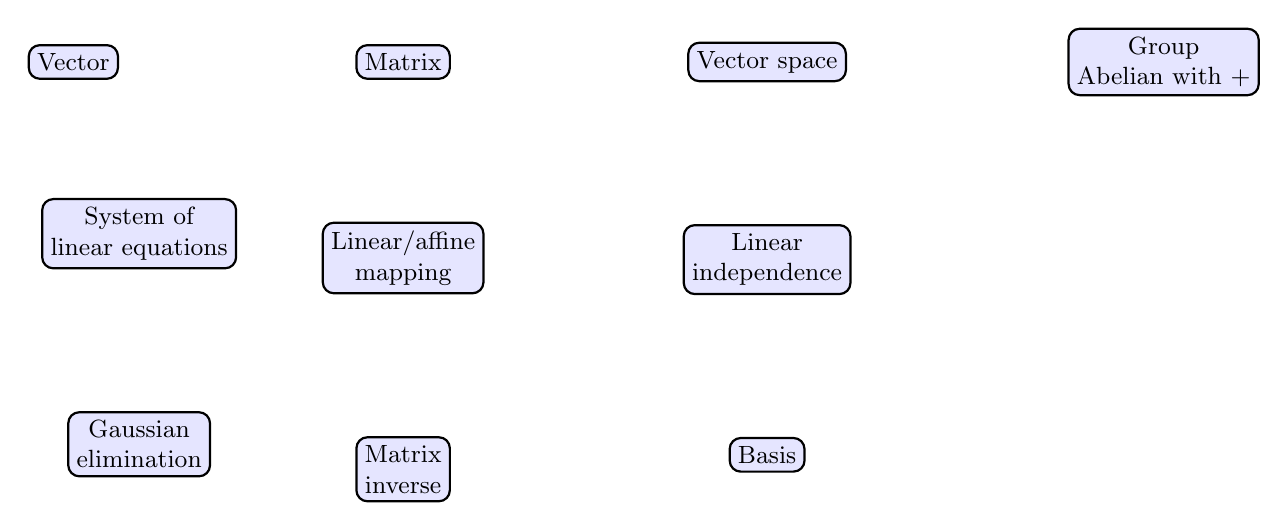
\begin{tikzpicture}[
  every node/.style={font=\small, align=center},
  box/.style={draw, rounded corners, fill=blue!10, inner sep=3pt},
  greenbox/.style={draw, rounded corners, fill=green!20, inner sep=3pt},
  ->, >=Latex, thick, node distance=1.5cm and 2cm
]

% Nodes
\node[box] (vector) {Vector};
\node[box, right=3cm of vector] (matrix) {Matrix};
\node[box, below=1.8cm of matrix] (linear_map) {Linear/affine\\ mapping};
\node[box, below left=1.5cm and 1.5cm of matrix] (system) {System of\\ linear equations};
\node[box, below=1.8cm of system] (gauss) {Gaussian\\ elimination};
\node[box, below=1.8cm of linear_map] (inverse) {Matrix\\ inverse};
\node[box, right=3cm of matrix] (vector_space) {Vector space};
\node[box, right=2.8cm of vector_space] (group) {Group\\ Abelian with +};
\node[box, below=1.8cm of vector_space] (indep) {Linear\\ independence};
\node[box, below=1.8cm of indep] (basis) {Basis};





\end{tikzpicture}

\end{document}
